\section{Localisation}
Localisation is the act of a robot finding out where it is. GPS systems are often used to do this in cases where precision is not critical, e.g. GPS navigation. If precision is critical, e.g. for a robot to drive past obstacles without hitting them, GPS is too imprecise. Other techniques must then be used. To do this, robots often have sensors, such as sonars, LIDARs or cameras. 
The localisation algorithms consists of two main parts, movement and measurement. Movement is imprecise, often because of the mechanical system. Measurements contributes with new knowledge and is therefore the part that narrows the decision, of where the robot is, in. The measurements is often also noisy, but usually less noisy than the movements.
Another important thing in localisation is probability. What is the probability of being in a certain position, given the measurement? To calculate this, Bayes rule is used.
\begin{equation}
p(x|z) = \frac{p(z|x)\cdot p(x)}{p(z)}
\end{equation}
Where $\frac{1}{p(z)}$ is the normalizing factor $\eta$.
\begin{equation}
\eta = \frac{1}{p(z)} = \frac{1}{\sum(p(z|x)\cdot p(x))}
\end{equation}
This gives us the expression:
\begin{equation}
p(x|z) = \eta \cdot p(z|x)\cdot p(x)
\end{equation}

\textbf{Eksample:}\\
A robot is in one of the grids in the map. It can detect if it is in a red or green grid. 
\begin{figure}[H]
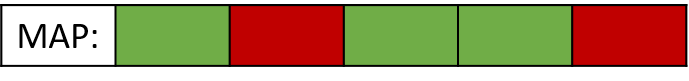
\includegraphics[scale=1]{billeder/Localisation01.png}
\caption{The map in which the robot lives}
\end{figure}
If the robot is in a green grid, it detects correctly with 75\% chance. If it is in a red grid, it detects correctly with 90\% chance.
If the robot detects green, what is the probability that it is in a green or a red grid?\\
$z = green$\\
$\eta = \frac{1}{sum(p(z|x)\cdot p(x))} = \frac{1}{0.75 \cdot \frac{3}{5} + 0.1 \cdot 2/5} = 2.04$\\\\
$x = green$\\
$p(x) = \frac{3}{5}$\\
$p(x \mid z) = \eta \cdot p(z|x)\cdot p(x) = 2.04 \cdot 0.75 \cdot \frac{3}{5} = 0.918 = 91.8\%$\\\\
$x = red$\\
$p(x) = \frac{2}{5}$\\
$p(x \mid z) = \eta \cdot p(z|x)\cdot p(x) = 2.04 \cdot 0.1 \cdot \frac{2}{5} = 0.082 = 8.2\%$

\subsection{Markov Localisation}
% Localisation_MarkovLocalisation
The purpose of Markov Localisation is to estimate where the robot is located, given its measurements, movements and a map describing the world in which the robot is placed.
Lets say the robot can move along a wall and sense whether if there is a door next to it or not. We place the robot in a world with a wall with 3 doors.
The estimation of the localisation of the robot is called belief and is the probability of being in a given location, given the previous act. At the beginning, the robot will not know where it is, and therefore it will have a uniformly distributed belief.\\ 
Then the robot takes a measurement, and let's say that it measures a door. Now the new belief is the former belief multiplied with the probability of the measurement z given the position x. 
\begin{equation}
bel'(x) = bel(x) \cdot p(z|x)
\label{ML_eq1}
\end{equation}
After this the robot moves. A movement is often noisy and therefore the precision of the belief will fall. This is illustrated by convolving the belief with the motion model. The motion model consists of a mean $\mu$, representing the noise free movement, and a standard deviation $\sigma$, representing the noise. The result of this step can be seen in \ref{ML_fig1:sub3}.
\begin{equation}
bel'(x) = bel(x) \ast norm(\mu,\sigma)
\label{ML_eq2}
\end{equation}
These two steps are now repeated the rest of the lifetime of the robot. Every time the robot senses, it gets more certain of where it is and every time it moves it gets more uncertain. In figure \ref{ML_fig1} two iterations are shown.

\begin{figure}[H]
\centering

\begin{subfigure}[b]{.8\textwidth}
  \centering
  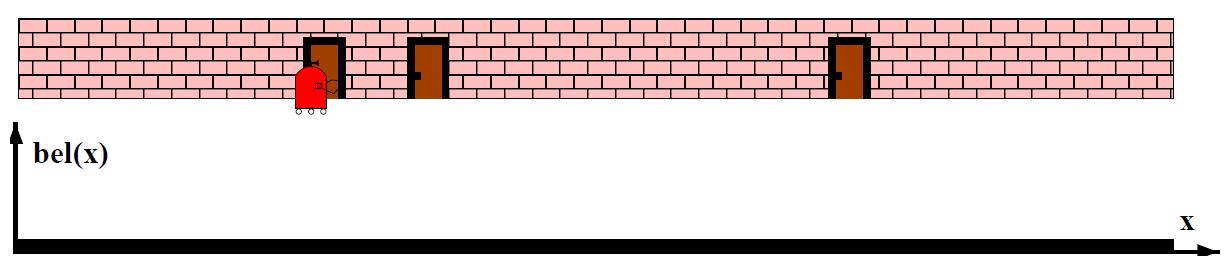
\includegraphics[width=1\linewidth]{billeder/MarkovLocalisation01.png}
  \caption{Initial belief is uniformly distributed.}
  \label{ML_fig1:sub1}
\end{subfigure}%

\begin{subfigure}[b]{.8\textwidth}
  \centering
  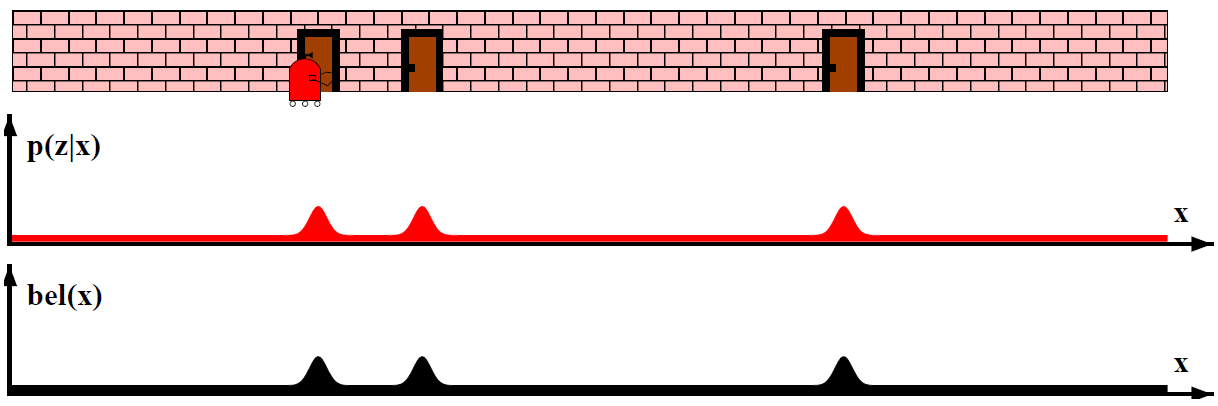
\includegraphics[width=1\linewidth]{billeder/MarkovLocalisation02.png}
  \caption{Measurement and result of belief multiplied with measurement.}
  \label{ML_fig1:sub2}
\end{subfigure}

\begin{subfigure}[b]{.8\textwidth}
  \centering
  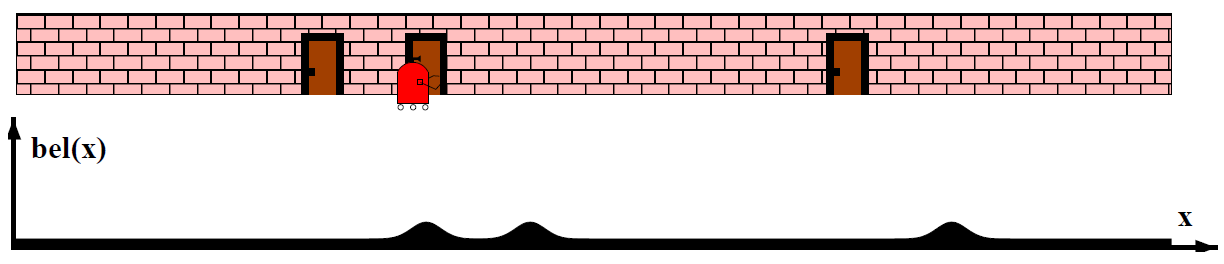
\includegraphics[width=1\linewidth]{billeder/MarkovLocalisation03.png}
  \caption{Movement of robot and belief. Noise makes the belief after the movement more uncertain.}
  \label{ML_fig1:sub3}
\end{subfigure}%

\begin{subfigure}[b]{.8\textwidth}
  \centering
  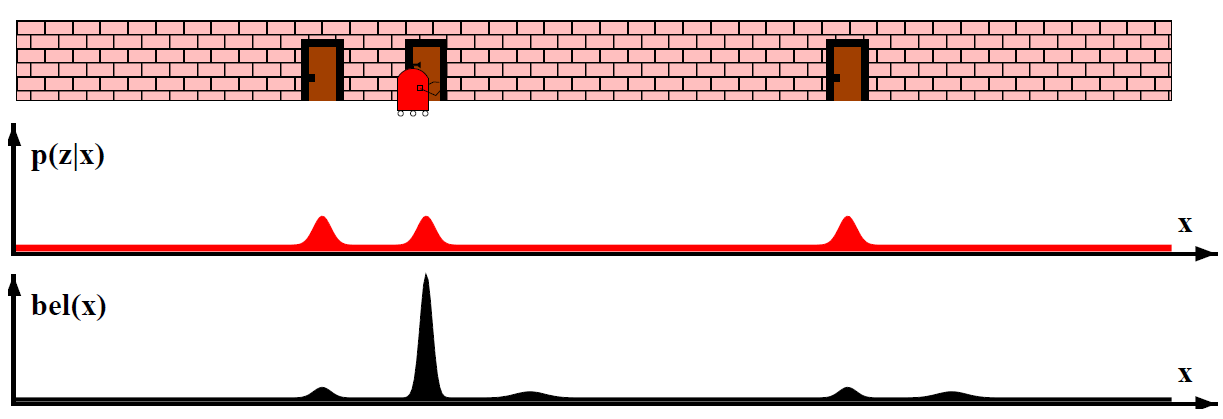
\includegraphics[width=1\linewidth]{billeder/MarkovLocalisation04.png}
  \caption{Measurement and result of belief multiplied with measurement.}
  \label{ML_fig1:sub4}
\end{subfigure}

\begin{subfigure}[b]{.8\textwidth}
  \centering
  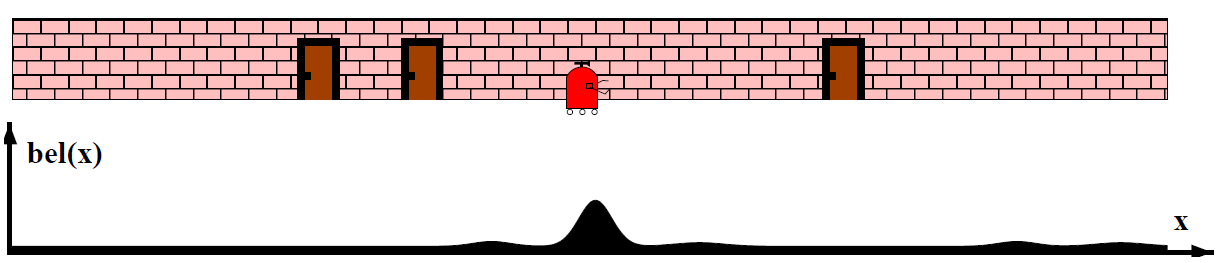
\includegraphics[width=1\linewidth]{billeder/MarkovLocalisation05.png}
  \caption{Movement of robot and belief. Noise makes the belief after the movement more uncertain.}
  \label{ML_fig1:sub5}
\end{subfigure}

\caption{Markov Localisation illustrated. \citep{thrun2005probabilistic}}
\label{ML_fig1}
\end{figure}

The algorithm for Markov Localisation is as follows:\\
1:\quad \textbf{Algorithm MarkovLocalization(}$bel(x_{t-1}),u_t,z_t,m$\textbf{):}\\
2:\quad \quad $for\,all\,x_t\,do$\\
3:\quad \qquad $\overline{bel}(x_t) = \int p(x_t|u_t,x_{t-1},m)\cdot bel(x_{t-1}) dx$\\
4:\quad \qquad $bel(x_t) = \eta p(z_t|x_t,m)\cdot \overline{bel}(x_t)$\\
5:\quad \quad $endfor$\\
6:\quad \quad $return\,bel(x_t)$

What happens is that after a move, $u_t$, and a measurement, $z_t$, has been taken, the algorithm is called. First it calculates the belief after the movement, and then it calculates the belief after the measurement. It does this for all possible places, $x_t$, in the map, $m$. This corresponds to the combinations of (a and b) or (c and d) in figure \ref{ML_fig1}.

\subsection{Kalman Filter}
The kalman filter is a method for sensor fusion. It is capable of taking two or more measurements and fuse together to one optimal guess of the true value. It does this by looking at the current measurement and comparing it with a predicted value. The predicted value is often a combination of the previous value combined with the changed done since the last measurement. 

The kalman filter has some limitations. One of them is that it assume that all noise in the system is Gaussian distributed, which is not always the case. Another is that it always gives only one guess on the value, which is optimal for a lot of systems but is not especially preferable in localisation. The last one is that it assumes that there is a linear relationship between all measurements and the value we are trying to estimate. 

Much like the Markov localisation the kalman filter have a measurement step, then it does some movement and predict the new value. This is done in a never ending continues process. 
\begin{figure}[H]
\centering
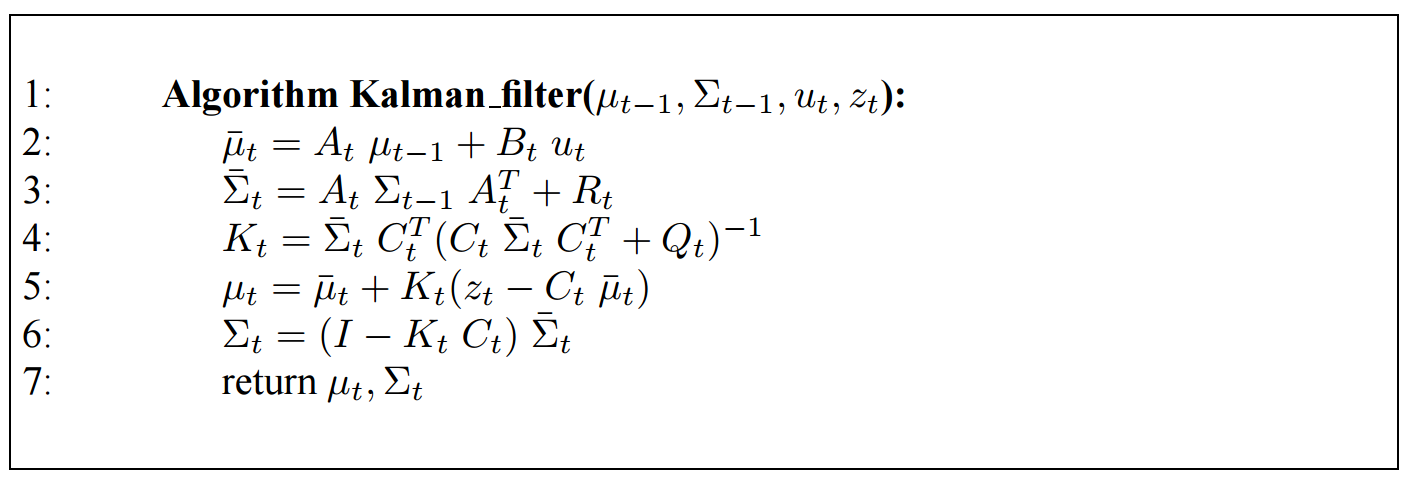
\includegraphics[width=1\textwidth]{billeder/KalmanFilter.png}
\caption{Kalman Filter algorithm}
\label{fig:kalmanfilter}
\end{figure}
If we look at the math, we can see that this can be done in a few steps. looking at the equations of the kalman filter we normally call 2-3 for the prediction step and 4-7 for the measurement step. 
\subsubsection{Prediction Step}
Looking at the equations in the prediction step (\ref{Pre1}, \ref{Pre2}).
\begin{gather}
\overline{\mu}_t = A_t \mu_{t-1} + B_t u_t
\label{Pre1}\\
\overline{\Sigma}_t = A_t \Sigma_{t-1} A^{\intercal}_t+ R_t
\label{Pre2}
\end{gather}
There are 2 conversion matrices $A$, $B$ and a measurement/input matrix $u$. The matrix $A$ must transform the last best estimate to the current domain. e.g. if we are trying to predict how far down a bungee jumper have fallen then the $A$ matrix must add the distance the gravity would have pulled him down since the last estimate $\mu_{t-1}$. We call this the static influence, since it is the change in the system if we do not interfere. The input matrix $u$ is the change we put in to the system since the last prediction. Lets say that we can increase or decrease the bungee jumpers air resistance. The $u$ matrix will contain the information about the change in air resistance. The $B$ matrix will convert the input matrix to the desired domain. For the bungee jumper it will convert air resistance to a fall distance. We call this the dynamic influence.
The last matrix $R$ is the noise, expressed as the covariance, of the input matrix $u$. This is to inform the system about the certainty of the input. 

As previously mentioned this dictates that there exists a linear conversion from the static and dynamic influences in relation to the the previous state to the new state. 
\subsubsection{Measurement Step}
Looking at the equations in the measurement step (\ref{Mes1}, \ref{Mes2} , \ref{Mes3}).
\begin{gather}
K_t = \overline{\Sigma}_t C^{\intercal}_t ( C_t \overline{\Sigma}_t C^{\intercal}_t + Q_t ) ^{-1} 
\label{Mes1} \\
\mu_{t} = \overline{\mu}_t +K_t (z_t-C_t\overline{\mu}_t) 
\label{Mes2} \\
\Sigma_t = (I-K_t C_t) \overline{\Sigma}_t 
\label{Mes3}
\end{gather}
The measurement step takes the predicted value $\overline{\mu}_t$, $\overline{\Sigma}_t$ and uses the measurement to fix the error in the prediction introduced by the noise. The measurement vector $z_t$ contains the measurement. For the bungee jumper it could be the tension in the bungee line. The conversion matrix $C_t$ convert the measurement to the value domain. So it takes the tension and convert to a distance. The $Q_t$ matrix is our measurement noise, expressed as the covariance.

By calculating the Kalman gain $K_t$ we get a kind of believe on the measurement, that decides how much we are able to affect the predicted value with information obtained from the measurement. 

After we have corrected the prediction, we have the best possible guess of the true value, or the true distance in the bungee case. 
\subsubsection{Graphical}
Looking at the bungee example, this can also be graphically shown. On figure \ref{bungeeFig} we see the bungee problem. 
\begin{figure}[H]
\centering
\includegraphics[width=1\textwidth]{billeder/Bungee.jpg}
\caption{The bungee problem}
\label{bungeeFig}
\end{figure}
First we see a the prediction step which have a very high uncertainty as shown with a Gaussian with a big variance. After this we make a measurement, as show in the second graph. we now use the kalman filter to estimate the best guess, based on the prediction and the measurement. 

We can see this as optimal fusion of our prediction information and our measurement information. 
\subsubsection{Kalman Filters In Robotics}
Like in the bungee example where the position of the bungee jumper was found. A robot can be located in a known map. 
But this is not the only use of a kalman filters in robotics.\\
Kalman filters are often used to fuse multiple sensor readings to one optimal guess, and to discover hidden variables. A hidden variable is a property that can not be directly measured, but have a relation to the measured data. lets say you can measure the location of a robot. Then the hidden variable can be the robots speed since the speed can be found looking at different locations over time. By using a kalman filter it is possible to estimate the speed very precise. \\
Since the kalman filter is uni-model, which mean that it only can give one guess of the location, other techniques, like particle filters and Markov localisation which gives multiple candidate locations, are often preferred. 
\subsubsection{Extended Kalman Filter}
One of the big limitations of the kalman filter is the requirement that dictates that there must be a linear relationship between measurements or input and the value domain. 

This limitation is removed in the extended kalman filter. This is done by replacing the linear conversion matrices $A$, $B$ and $C$ with the none linear functions $g(u_t, \mu_{t-1})$ and $h(\overline{\mu}_t)$.\\

Since the kalman filter basically exploits the principle of a Gaussian converted with a linear transformation still is a Gaussian. Introducing the non linear functions brakes the filter. To fix this the extended kalman filter utilize a method called first order Taylor expansion. Taylor expansion construct a linear approximation to a function, in a given point. This is done by using the partial derivative of the function in the point. We create the partial derivative matrices $G$ and $H$.
\begin{equation}
G = \frac{\partial g(u_t, \mu_{t-1})}{\partial \mu_{t-1}} \\ H = \frac{\partial h(\overline{\mu}_t)}{\partial \overline{\mu}}
\end{equation}
We can now use this in the regular kalman filter to obtain the extended kalman filter.
\begin{figure}[H]
\centering
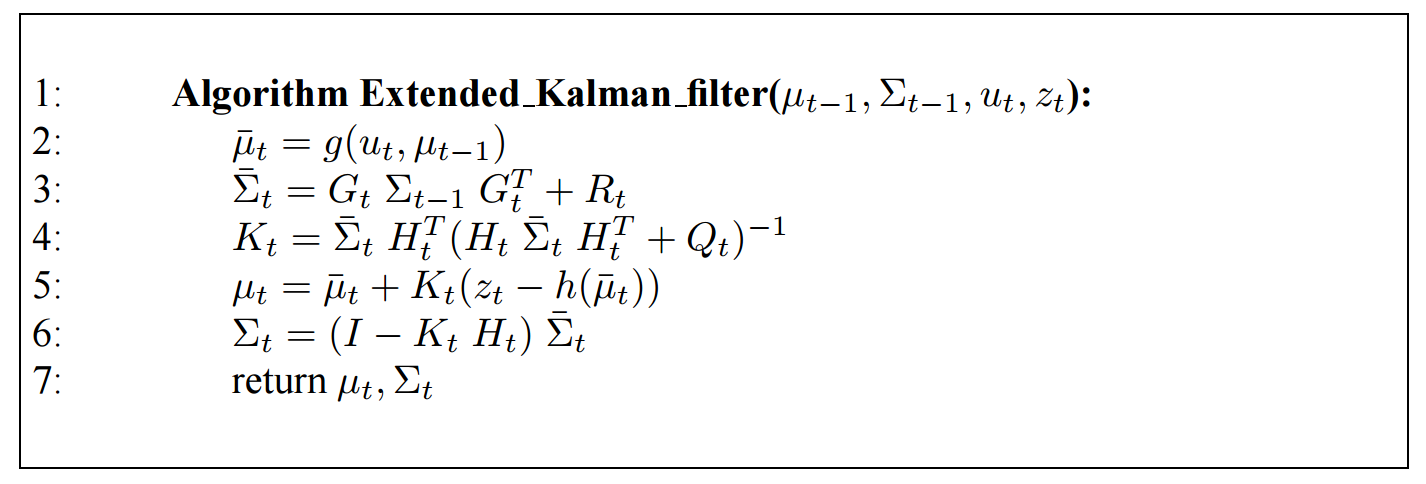
\includegraphics[scale=0.51]{billeder/EKF.png}
\caption{Extended Kalman Filter algorithm}
\end{figure}
It has been shown that this type of kalman filter is far better in practice than the regular kalman filter if the variance of prediction and measurement is small. If this is not the case the linearisation introduces additional noise. This is due to the error between the linearisation and the true function. The greater the variance the greater impact it has.  



\subsection{Particle Filter}
The particle filter is a different kind of filter, since it uses a discrete method for finding the robots location, in contrast to the continuously methods previously discuses. \\
The method is multi-model, which means that more than one location candidate can be found. This is a very popular technique for localisation, since it is simple to understand and implement. 
\\
\\
Like the other filters, the particle filter does also require the map to be known, and we must be able to predict how all measurements will look in any given location. 

The particle filter can also be seen as having a prediction step and a measurement step. Before we start the measurement-prediction loop, we first select a number $M$ of particles $X$ to use in the filter. Then we place all the $M$ particles at random locations. 

\subsubsection{Prediction Step}
After the robot have moved with a motion $u_t$, we move all the particles with the same motion. On this motion we add some random noise $w_t$. If one of the particles was exactly at the robot location before we moved it, and the noise we put on the particle was the exact same as on the real robot, the new particle location would still be the same as the robot.  

\subsubsection{Measurement Step}
First we take the measurement from the real robot $z_t$. Then we compare it to all of the $M$ particles and calculate the probability off the location of the real robot is the same as for the particle. This is done by comparing the measurement $z_t$, with the measurement that would have been at the particle location.
At this process it is important to assume that there is noise on the measurements. If we assume that the sensor is to precise we risk giving particles that are close to the real location a low probability, which is not desirable.\\\\
When we have all the probabilities for the particles $Prob_t$, we are doing resampling. The aim of resampling is to get a new set of $M$ new particles. The locations of the new particles must be randomly drawn from the old particle set whit a distribution that matches the $Prob_t$ distribution. This means that a lot of the new particles are at the locations with high probability, where only a few or none is at locations with low probability.\\ 
\\
After the resampling we continue with the prediction step, and so one. 

\subsubsection{The Algorithm}
Over time particles with at bad locations will die, and more will search the area around feasible locations. The predict - measurement steps can also be expressed as pseudo code as seen below: 

\begin{figure}[H]
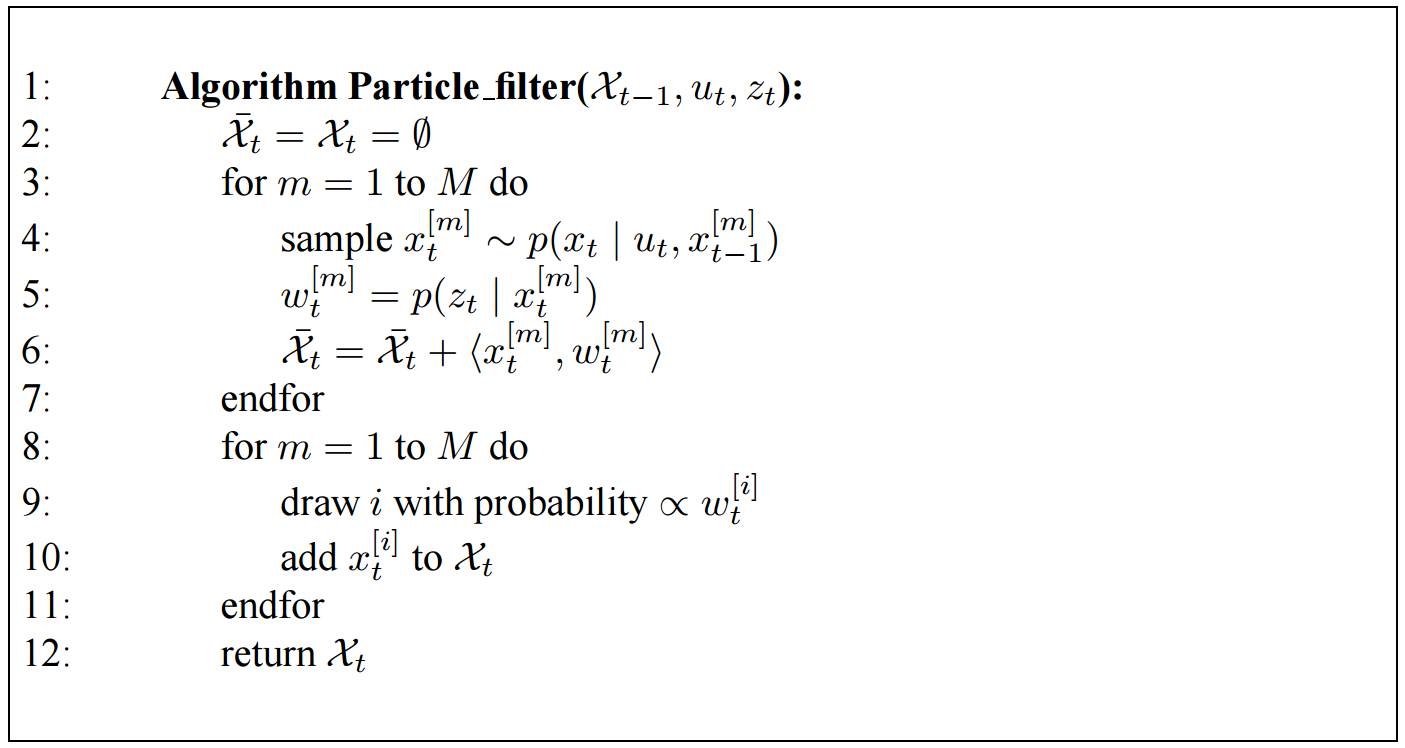
\includegraphics[scale=0.51]{billeder/ParticleFilter.png}
\end{figure}

This process runs continuously, and will over time converge to zero or one single location.

\subsubsection{Particle Filters Considerations}
A series of scenarios must be considered when using particle filters. One is the scenario where there is not placed a particle close to the real robot or all the particles around it dies. This will make the particle filter coverage around a wrong location or no location. There are several techniques tackling this problem. One easy simple solution is to look at probability and see if there is at least one good candidate. If this is not the case the filter should be reset. 
\\\\
One other problem happens if the world is symmetric, this means that every measurement have multiple feasible locations, and when moved previously feasible locations still appearers equally likely. If this is the case it is impossible to know the true location. This is can also in extreme cases be a problem if the world is only partially symmetric, since all the true particles can die, and only the wrong survive. When we now enter a asymmetric area all the wrong will die, and we have no particles left. This can be fixed by either resetting the filter, or by a technique where you all ways randomly spread out the worst $5\%$ of you particles. 
\\\\
Also a balance must be found with the number of particles and the map size. The more particles the better the filter, but it will also drastically increase the calculation time. 

%------------------------------------------------